\documentclass[tikz,border=4pt]{standalone}
\usepackage{xcolor}
\definecolor{journalink}{HTML}{1F1C18}
\begin{document}
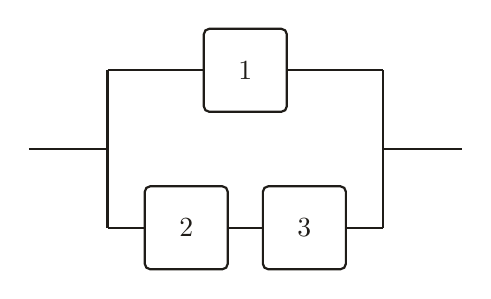
\begin{tikzpicture}[-,auto,node distance=1cm,
  point/.style={coordinate},
  block/.style={draw=journalink, line width=0.8pt, rounded corners=2pt, rectangle, minimum height=3em, minimum width=3em, text=journalink},
  every path/.style={draw=journalink, line width=0.8pt}]
\node[point] (0) at (-0.5,0)  {};
\node[point] (1) at (0.5,0)  {};
\node[point] (2) at (0.5,1)  {};
\node[block] (3) at (2.25,1)  {1};
\node[point] (4) at (4,1)  {};
\node[point] (5) at (0.5,-1)  {};
\node[block] (6) at (1.5,-1)  {2};
\node[block] (7) at (3,-1)  {3};
\node[point] (10) at (4,-1)  {};
\node[point] (8) at (4,0)  {};
\node[point] (9) at (5,0)  {};
\draw   (0) -- (1);
\draw   (1) -- (2);
\draw   (1) -- (5);
\draw   (2) -- (3);
\draw   (3) -- (4);
\draw   (5) -- (6);
\draw   (6) -- (7);
\draw   (7) -- (10);
\draw   (4) -- (8);
\draw   (10) -- (8);
\draw   (8) -- (9);
\end{tikzpicture}
\end{document}
